\documentclass{beamer}
\usepackage[polish]{babel}
\usepackage[utf8]{inputenc}
\usepackage{lmodern}
\usepackage{enumerate}
\usepackage{listings}
\usepackage{color} %red, green, blue, yellow, cyan, magenta, black, white
\definecolor{mygreen}{RGB}{28,172,0} % color values Red, Green, Blue
\definecolor{mylilas}{RGB}{170,55,241}

\usetheme{AGH}

\title{Projektowanie układów regulacji za pomocą linii pierwiastkowych}
\subtitle{Podstawy Automatyki}
\author{Piotr Kucharski i Dominik Zabłotny}
\website{\url{https://github.com/AGH-Kucharski-Zablotny/Podstawy-Automatyki}}
\institute{Wydział Elekrotechniki, Automatyki, Informatyki i Inżynierii Biomedycznej}
\date{\today}

\lstset{
language=Matlab,%
basicstyle=\tiny,
breaklines=true,%
morekeywords={matlab2tikz},
keywordstyle=\color{blue},%
morekeywords=[2]{1}, keywordstyle=[2]{\color{black}},
identifierstyle=\color{black},%
stringstyle=\color{mylilas},
commentstyle=\color{mygreen},%
showstringspaces=false,%without this there will be a symbol in the places where there is a space
numbers=left,%
numberstyle={\tiny \color{black}},% size of the numbers
numbersep=9pt, % this defines how far the numbers are from the text
emph=[1]{for,end,break},emphstyle=[1]\color{red}, %some words to emphasise
%emph=[2]{word1,word2}, emphstyle=[2]{style},  
}

\begin{document}

\titleframe[pl]

\begin{frame}\frametitle{Zadanie 2}\framesubtitle{Dobór regulatora proporcjonalnego}
	Dany jest układ:
	\[
	G(s) = \frac{1}{s(s+1)(0.2s+1)}
	\]
    \begin{enumerate}[a)]
        \item Wykorzystując poznane narzędzia dobierz regulator proporcjonalny (wzmocnienie K) aby układ zamknięty miał współczynnik tłumienia $\xi = 0.707$ (wtedy $\phi = 45\degres$). Narysuj odpowiedź skokową układu zamkniętego.
        
        \centering{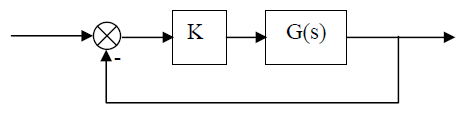
\includegraphics[scale=0.65]{uklad_2.png}}
        
        %\item Dodaj do układu kompensator (człon przyspieszająco-opóźniający fazę) o transmitancji:
        %\[
        %	G_c(s) = \frac{(s+1)}{(0.1s+1)}
        %\]
        %czyli utwórz następujący układ:
    \end{enumerate}
\end{frame}

\begin{frame}[fragile]\frametitle{Zadanie 2a}\framesubtitle{Dobór regulatora proporcjonalnego - algorytm i kod}
	\begin{lstlisting}
% Utworzenie ukladu dynamicznego
sys = zpk([],[0 -1 -5], 5);

% Narysowanie linii pierwiastkowych
rlocus(sys);

% Pomocnicza linia pod zadanym katem 45 stopnii
line([0 -15], [0 15]);           

% Zatrzymanie w celu przyblizenia
pause();                            

% Obliczenie K dla zadanego kata
[K, bieguny] = rlocfind(sys);       

% Zamkniecie ukladu dynamicznego
sys_zamk = feedback(K * sys, 1);    

% Odpowiedz ukladu zamknietego na skok jednostkowy
step(sys_zamk);                     
	\end{lstlisting}
\end{frame}

\begin{frame}\frametitle{Zadanie 2a}\framesubtitle{Dobór regulatora proporcjonalnego - wykonanie}
\centering	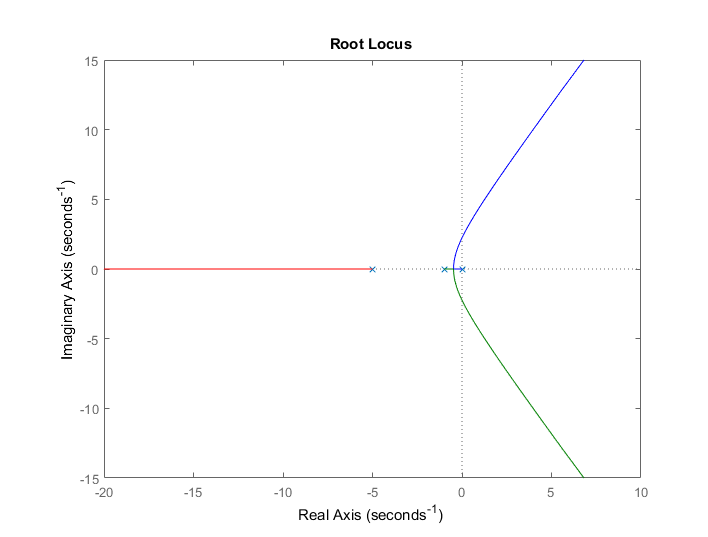
\includegraphics[scale=0.5]{a-rlocus-bez-linii.png}
\end{frame}

\begin{frame}\frametitle{Zadanie 2a}\framesubtitle{Dobór regulatora proporcjonalnego - wykonanie}
\centering	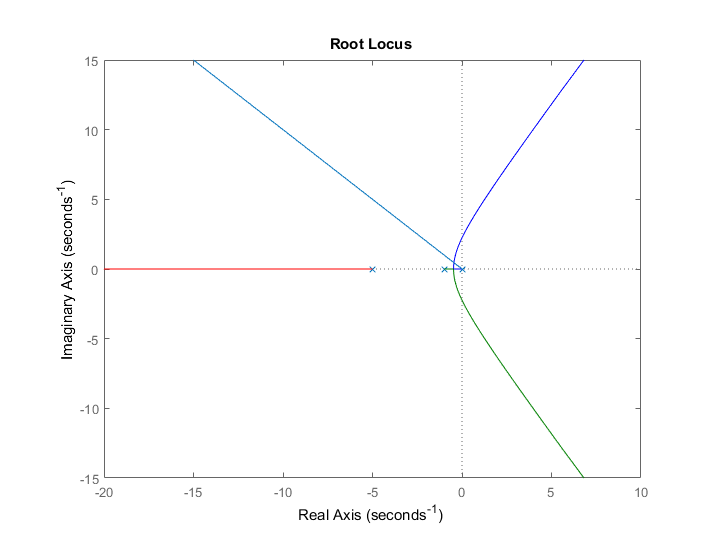
\includegraphics[scale=0.5]{a-rlocus.png}
\end{frame}

\begin{frame}\frametitle{Zadanie 2a}\framesubtitle{Dobór regulatora proporcjonalnego - wykonanie}
\centering	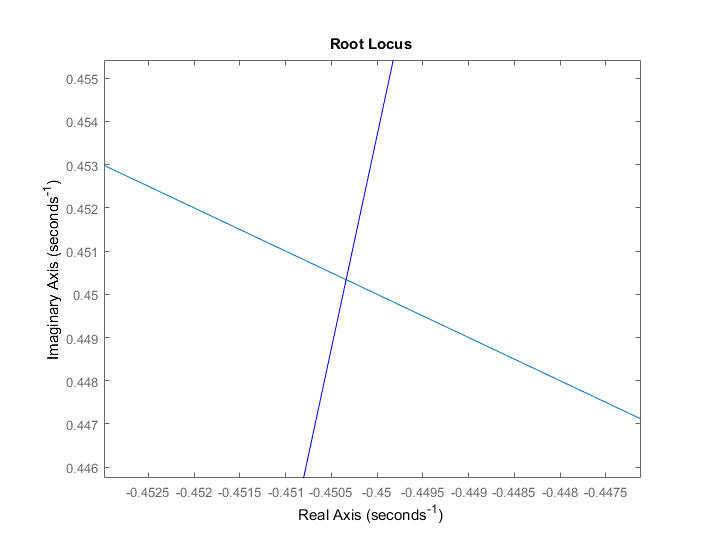
\includegraphics[scale=0.5]{a-przyblizenie.png}
\end{frame}

\begin{frame}\frametitle{Zadanie 2a}\framesubtitle{Dobór regulatora proporcjonalnego - wykonanie}
\centering	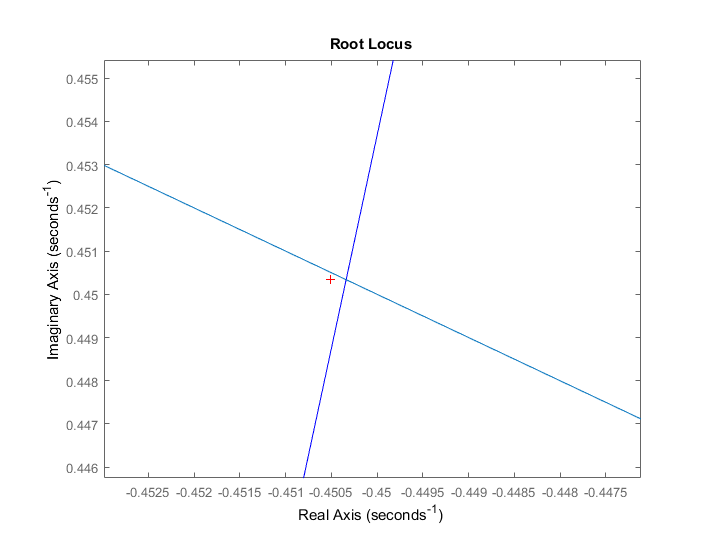
\includegraphics[scale=0.5]{a-rlocfind.png}
\end{frame}

\begin{frame}\frametitle{Zadanie 2a}\framesubtitle{Dobór regulatora proporcjonalnego - wykonanie}
\centering	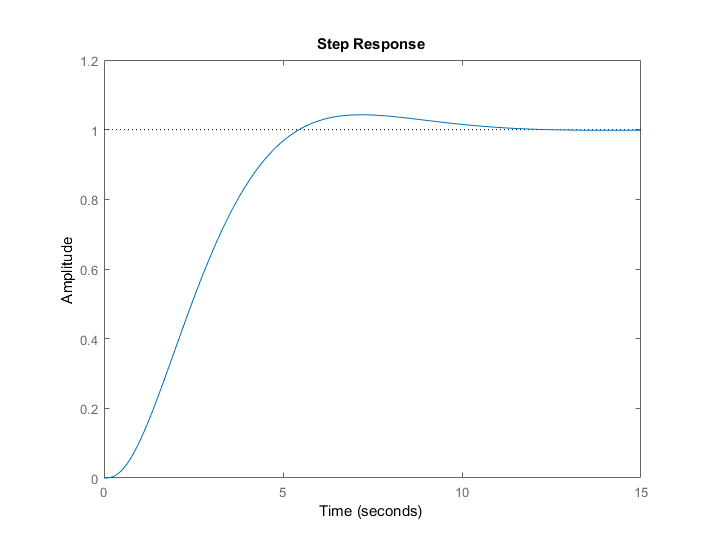
\includegraphics[scale=0.5]{a-sys-zamk.png}
\end{frame}

%-----------B------------

\begin{frame}\frametitle{Zadanie 2b}\framesubtitle{Dobór regulatora proporcjonalnego z kompensatorem}
	\begin{enumerate}[b)]
		
	\end{enumerate}
\end{frame}

\begin{frame}[fragile]\frametitle{Zadanie 2b}\framesubtitle{Dobór regulatora proporcjonalnego z kompensatorem - algorytm i kod}
	\begin{lstlisting}
% Oryginalny system dynamiczny
sys = zpk([],[0 -1 -5], 5);
% Utworzenie kompensatora
Gc = zpk(-1, -10, 1/10);
% Utworzenie systemu zastepczego
system_zastepczy = series(sys, Gc);
% Narysowanie linii pierwiastkowych ukladu zastepczego
rlocus(system_zastepczy);
% Narysowanie linii pomocniczej
line([0, -15], [0, 15]);
% Zatrzymanie wykonywania w celu przyblizenia
pause();
% Obliczenie wzmocnienia dla ukladu zastepczego
[K, bieguny] = rlocfind(system_zastepczy);
% Stworzenie ukladu zamknietego
sys_zamk_b = feedback(K * system_zastepczy, 1);
% Odpowiedz ukladu zastepczego na skok jednostkowy
step(sys_zamk_b);
	\end{lstlisting}
\end{frame}

\begin{frame}\frametitle{Zadanie 2b}\framesubtitle{Dobór regulatora proporcjonalnego z kompensatorem - wykonanie}
\centering	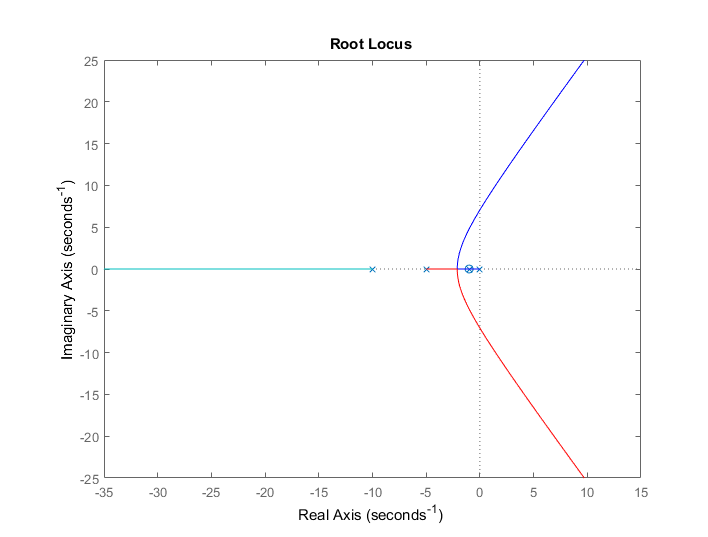
\includegraphics[scale=0.5]{b-rlocus-bez-linii.png}
\end{frame}

\begin{frame}\frametitle{Zadanie 2b}\framesubtitle{Dobór regulatora proporcjonalnego z kompensatorem - wykonanie}
\centering	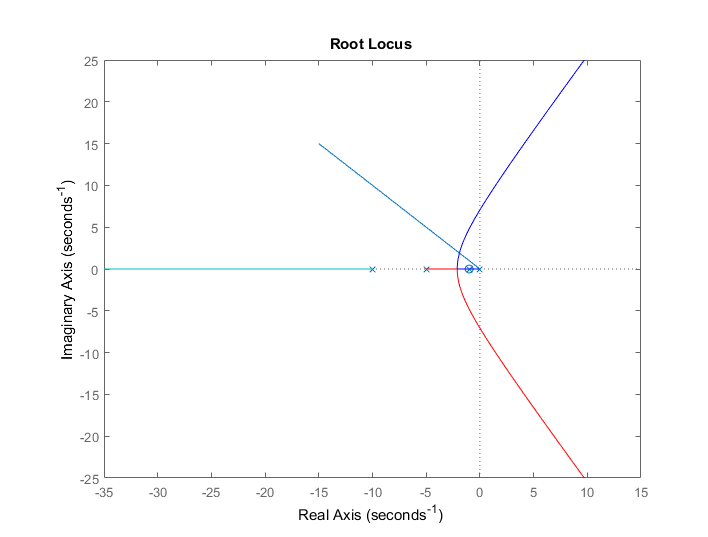
\includegraphics[scale=0.5]{b-rlocus.png}
\end{frame}

\begin{frame}\frametitle{Zadanie 2b}\framesubtitle{Dobór regulatora proporcjonalnego z kompensatorem - wykonanie}
\centering	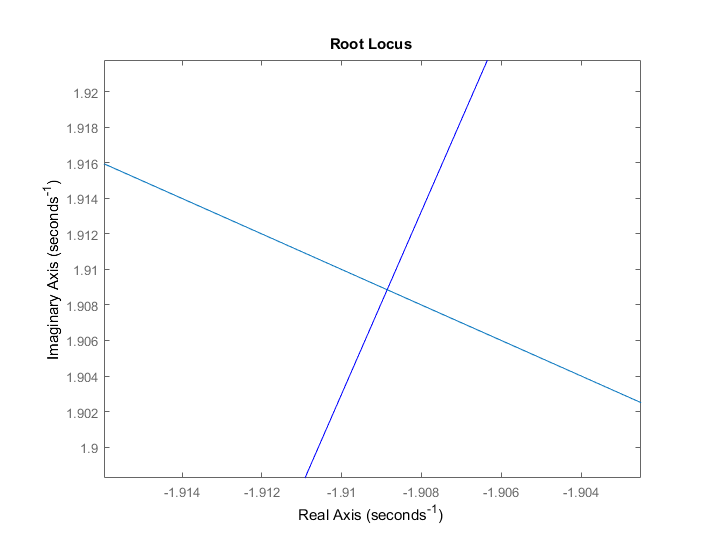
\includegraphics[scale=0.5]{b-przyblizenie.png}
\end{frame}

\begin{frame}\frametitle{Zadanie 2b}\framesubtitle{Dobór regulatora proporcjonalnego z kompensatorem - wykonanie}
\centering	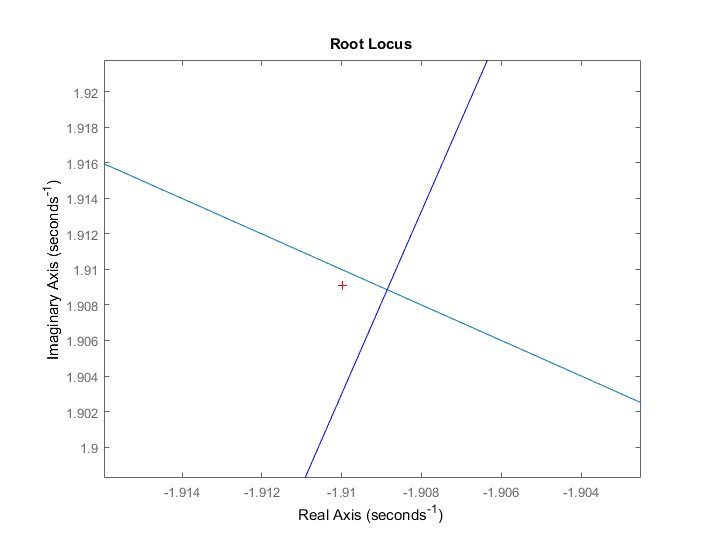
\includegraphics[scale=0.5]{b-rlocfind.png}
\end{frame}

\begin{frame}\frametitle{Zadanie 2b}\framesubtitle{Dobór regulatora proporcjonalnego z kompensatorem - wykonanie}
\centering	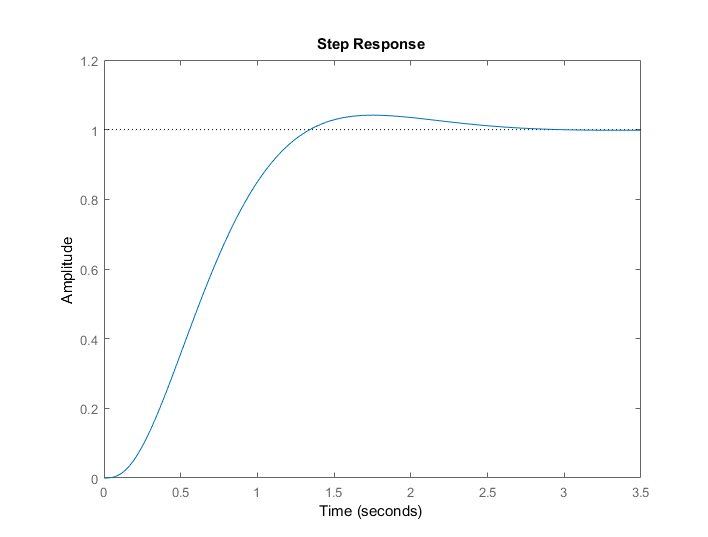
\includegraphics[scale=0.5]{b-sys-zamk.png}
\end{frame}

%------------OBA-------------
\begin{frame}\frametitle{Zadanie 2}\framesubtitle{Dobór regulatora proporcjonalnego - porównanie}
\centering	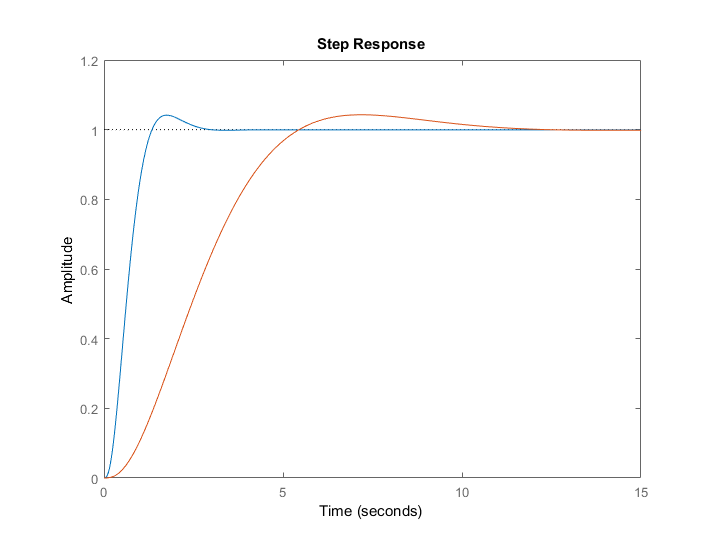
\includegraphics[scale=0.5]{step-oba.png}
\end{frame}


\end{document}
